\section{Потенциалы. Силовые линии и эквипотенциальные поверхности}

	Покажем, что электрическая сила консервативна \index{Сила!электрическая}. В силу принципа суперпозиции \index{Принцип!суперпозиции}
		$$\vec{E}=\sum_i \vec{E}_i,$$
	откуда
		$$A=\sum_i A_i.$$
	Поле электрического заряда центрально симметричное \index{Поле!центрально симметричное}, следовательно работа \index{Работа} электрических сил по замкнутому контуру равна нулю:
		$$\oint \vec{F}\cdot\dvec\vec{l}=q\oint \vec{E}\cdot\dvec\vec{l}=0.$$
	Если есть консервативная сила, то есть и потенциальная энергия \index{Энергия!потенциальная}. Например, силе $\vec{F}_{\text{грав}}=G\dfrac{m_1m_2\vec{r}}{r^3}$ соответствует потенциальная энергия $E=-G\dfrac{m_1m_2}{r}$. Рассуждая аналогично, определим \i{потенциальную энергию электрического поля, порождаемого зарядом}:
		\begin{equation}
			E_{\text{п}}=+k\frac{q_1q_2}{r}.
		\end{equation}
	В соответствии с~принципом суперпозиции
		$$E_{\text{п}}=\sum_i E_i=\sum_i k\frac{qq_i}{r_i}=q\sum_i k\frac{q_i}{r_i}.$$
	Скалярную величину $\varphi=\dfrac{E_{\text{п}}}{q}$ назовем \i{электрическим потенциалом точки} \index{Потенциал}.
		$$\dim{\varphi}=\frac{\text{Дж}}{\text{Кл}}=\text{В (вольт)}.$$
	Для потенциала также выполняется принцип суперпозиции \index{Принцип!суперпозиции}:
		$$\varphi=\sum_i \varphi_i=\sum_i k\frac{q_i}{r_i}.$$
	Потенциал действует на заряды \index{Заряд} и создается зарядами. Знак потенциала соответствует знаку зарада, его породившего. \par
	Пусть заряд $q$ передвигается в~электрическом поле \index{Поле!электрическое} из точки 1 в 2. Тогда работа \index{Работа} электрической силы запишется как
		$$A=E_{\text{п}_{\text{1}}}-E_{\text{п}_{\text{2}}}=q\varphi_1-q\varphi_2=q(\varphi_1-\varphi_2).$$
	Назовем величину $U=\varphi_1-\varphi_2$ \i{напряжением} \index{Напряжение} и запишем работу $A$ в виде
		\begin{equation}
			A=qU.
		\end{equation}
	Заряд $q$ называется \i{пробным} \index{Заряд!пробный}, если он достаточно мал, чтобы в~условии данной задачи не~менять распределение и~картину поля от~всех остальных зарядов.\par
	Для визуального представления полей использутся силовые линии\index{Линия!силовая}~--- воображаемые линии, в~каждой своей точке сонаправленные с~вектором \index{Вектор!напряженности электрического поля} напряженности электрического поля в~этой точке. Густота\index{Густота}~--- величина $\Gamma=\dfrac{N}{S}$~--- это отношение числа $N$ силовых линий, проходящих через единицу площади $S$, к~$S$; иначе говоря, густота~--- это <<плотность>> силовых линий.\par
	\i{Эквипотенциальная поверхность}\index{Поверхность!эквипотенциальная}\index{Эквипотенциал}~--- это множество точек пространства, имеющих одинаковый потенциал.
	
	\subsection{Связь поля с потенциалом} 	

		Мы показали, что работа \index{Работа} по перемещению заряда $q$ в электрическом поле равна
			$$A=q\left(\varphi_1-\varphi_2\right).$$
		С другой стороны,
			$$A=\int\limits_1^2\vec{F}\cdot\dvec\vec{l}=q\int\limits_1^2\vec{E}\cdot\dvec\vec{l},$$
		тогда
			$$\left(\varphi_1-\varphi_2\right)=\int\limits_1^2\vec{E}\cdot\dvec\vec{l}=\int\limits_1^2 E\cos{\alpha}\d l=\int\limits_1^2 E_l\d{l}.$$
		При малых $l$ верно, что
			$$-\d\varphi=E_l\d{l},$$
		откуда
		\begin{equation}
			E_l=-\frac{\d\varphi}{\d l}.
		\end{equation}
		В пространстве соответственно имеем
			$$E_x=-\frac{\d\varphi}{\d x}, \quad E_y=-\frac{\d\varphi}{\d y}, \quad E_z=-\frac{\d\varphi}{\d z},$$
		что также можно записать в виде \index{Градиент}
			$$\vec{E}=-\grad{\varphi}.$$
		Все эти соображения наводят на новую размерность \index{Размерность} напряженности $E$:
			$$\dim{E}=\frac{\text{В}}{\text{м}}.$$

	\subsection{Свойства силовых линий и эквипотенциальных поверхностей}
		\begin{enumerate}
			\item Силовые линии не~пересекаются \index{Линия!силовая}.
			\item Электрическое поле \index{Поле!электрическое} перпендикулярно эквипотенциальной поверхности\index{Поверхность!эквипотенциальная}. Возьмем пробный заряд \index{Заряд!пробный} и~перенесем его вдоль эквипотенциальной поверхности. Запишем работу\index{Работа}, совершенную полем:
				$$A=qE\d{l}\cos{\alpha}=-q\d{\varphi} = 0, \quad E\cos{\alpha}=0,$$
				следовательно, вектор напряженности \index{Вектор!напряженности электрического поля} перпендикулярен эквипотенциальной поверхности, а~при перемещении заряда вдоль нее поле не~совершает работу.
			\item Силовое поле направлено в сторону уменьшения потенциала.
			\item Силовая линия \index{Линия!силовая} не пересекает эквипотенциальную поверхность дважды.
			\item В~точках пересечения эквипотенциальных поверхностей поле равно нулю; иначе говоря, поле равно нулю там, куда нельзя провести перпендикуляр.
			\item В силу центральной симметрии поля \index{Симметрия!центральная}, порождаемого точечным зарядом \index{Заряд!точечный}, эквипотенциальные поверхности имеют форму сферы.
					\begin{figure}[h!]
						\centering
						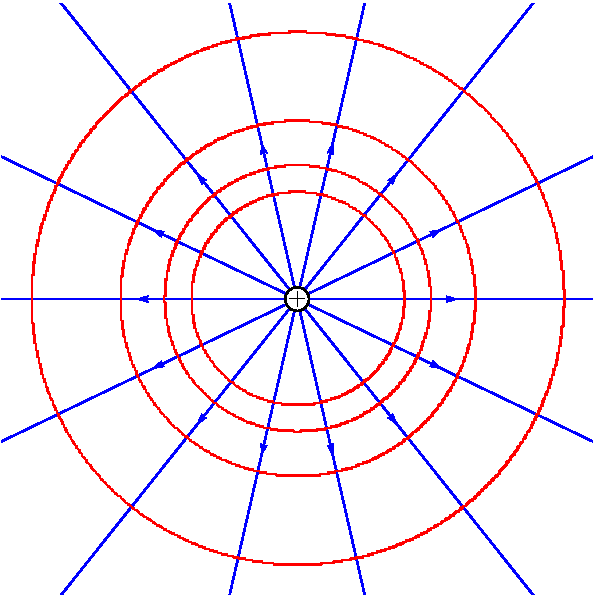
\includegraphics[scale=0.75]{./img/fig14/fig14.pdf}
						\caption{Положительный заряд, его поле и эквипотенциальные поверхности}
					\end{figure}
					\begin{figure}[h!]
						\centering
						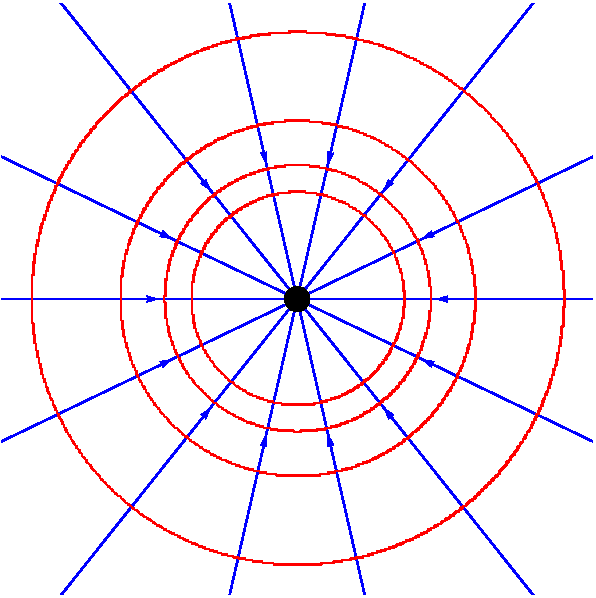
\includegraphics[scale=0.75]{./img/fig15/fig15.pdf}
						\caption{Отрицательный заряд, его поле и эквипотенциальные поверхности}
					\end{figure}

			\item Силовые линии \index{Линия!силовая} не могут начинаться в пространстве нигде, кроме как в точках положительных зарядов, и заканчиваться нигде, кроме как в точках отрицательных.
		\end{enumerate}
